\documentclass[a4paper, twocolumn]{article}
\newcommand{\papertitle}{Whitepaper: Community Development of Next Generation Storage and Compute Interfaces}

\usepackage[a4paper, margin=2cm]{geometry}

\usepackage[utf8]{inputenc}
\usepackage[T1]{fontenc}
\usepackage{graphicx}
\usepackage[english]{babel}
\usepackage[colorlinks=true,urlcolor=red]{hyperref}
\usepackage{url}
\usepackage{cleveref}

\usepackage{multicol}
\setlength{\columnsep}{1cm}

\usepackage{fancyhdr}
\fancyhead{}
\fancyfoot{}
\fancyhead[l]{\papertitle}
\fancyhead[r]{
\includegraphics[height=1em]{ngi-logo}}
\fancyfoot[r]{\thepage}
\pagestyle{fancy}
\renewcommand{\headrulewidth}{1pt}
\renewcommand{\footrulewidth}{1pt}

\usepackage{titling}
\pretitle{\begin{center}\Large\bfseries}
\posttitle{\end{center}\vskip 0.5em}

\graphicspath{{./assets/}}

\title{\papertitle}

\author{Julian M. Kunkel \\
  \textit{University of Reading}
	\and
  A
  \and
  B
  \and
  C
}
\date{\today}


\begin{document}
\maketitle
\thispagestyle{fancy}

\section*{Abstract}

The efficient, convenient, and robust execution of data-driven workflows and enhanced data management are key for productivity in scientific computing and computer-aided RD\&E.
Big data tools integrate compute and storage capabilities into a holistic solution demonstrating the benefit of tight integrating while the HPC community still optimizes the compute and storage components independently from each other, and, moreover, independently from the needs of end-to-end workflows from users that lead to the final insight.
Utilizing a homogeneous storage and compute infrastructure efficiently is complex for experts even when staying within the data center.
However, the execution of individual tasks from workflows may benefit from alternative hardware architectures and infrastructures -- the efficient management of data and compute capabilities in such a heterogeneous environment is an unresolved question.
In this white paper, we describe the vision for the Next-Generation Interface (NGI) initiative that aims to tackle the aforementioned storage and compute challenges in a holistic.
Within the NGI consortium, we fuse state-of-the-art concepts into a revolutionary approach by adding key features that increase opportunities for smarter scheduling of compute and storage in heterogeneous environments considering characteristics of workflows and data.
From the user perspective, NGI aims to provide an abstraction to data-driven processing and data management.
From the system perspective, NGI aims to derive an execution plan that utilizes the available hardware and software infrastructure within and across data centers.

\section{Introduction}

\subsection{Heterogeneous Systems}

The variety of tasks executed by a single workflow may benefit from a heterogeneous storage and compute infrastructure and potentially even spanning multiple locations.
\Cref{fig:heterogeneous} focuses on the computation in server nodes and storage of such an environment.
A variety of accelerators (GPU, TPU, FPGAs), active storage, in-memory, and in-network computing technologies provide processing capabilities across an HPC center optimized for certain workloads.
Data centers typically provide more than one storage class with different characteristics to optimize cost and efficiency.
Likewise, storage is deployed in the data center wide, locally available to individual nodes or subsets (e.g., racks); depending on the need, the characteristics range from predictable low-latency (in-memory storage, NVMe) to online storage (SSD, HDD), to cheap storage for long-term archival (tape).

The processing across geographic locations is nowadays mandatory to tame the data volumes of observational or simulation data.
Also, the lines between cloud computing and HPC are blurry, attempts are made to augment processing by flexibly migrate bursts of compute to cloud environments, ingest data from the cloud or store intermediate products for the final processing in clouds.
Consider a simple scenario where sensor data captured is pre-processed (cleaned) locally, then enriched with an additional data source in a small-scale HPC facility or by using fog computing, then transferred to a data center that performs the number crunching and generating data products.
These data products may be processed further in the cloud.

Utilizing the compute and storage characteristics of such a heterogeneous environment is challenging.
Manual and hard-coded workflows cannot handle changes in the environment and are error prone.
Therefore, users must be able to express their workflows in an abstract fashion that allows the system to generate (near-)optimal execution plans and monitor their execution.


\begin{figure}[b]
  \centering
  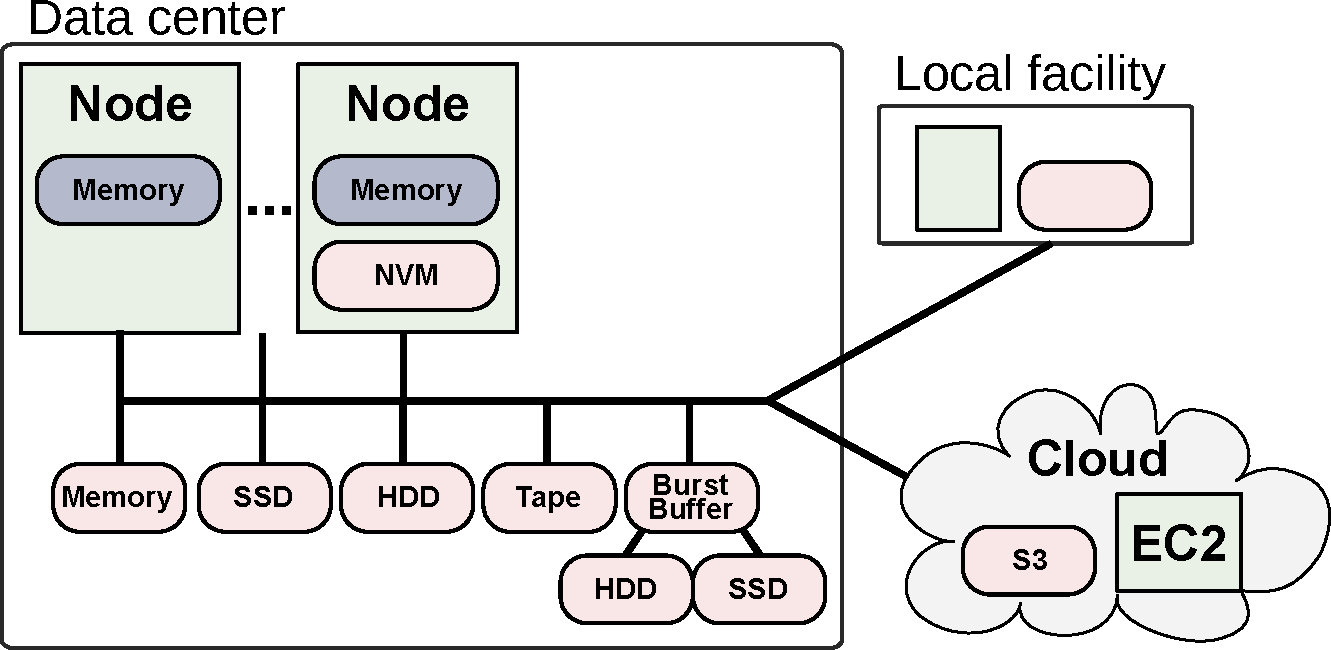
\includegraphics[width=\columnwidth]{system}
  \caption{Example Heterogeneous HPC Landscape}
  \label{fig:heterogeneous}
\end{figure}



\subsection{Experimental Planning}

Workflows, experimental design to result production.

Simulation

\Cref{fig:workflow}

\begin{figure}[b]
  \centering
  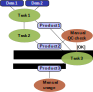
\includegraphics[width=0.75\columnwidth]{workflow}
  \caption{Example High-Level Workflow without Characteristics}
  \label{fig:workflow}
\end{figure}



\begin{figure}[b]
  \centering
  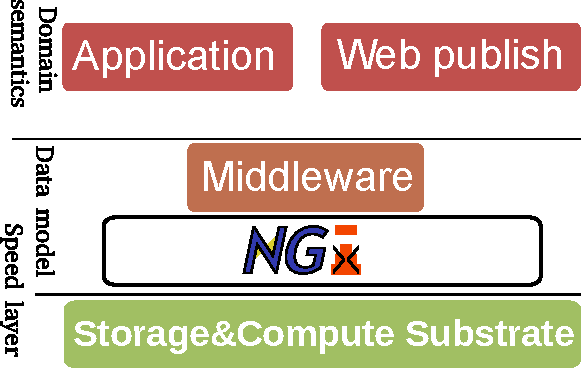
\includegraphics[width=0.75\columnwidth]{layers-ngi}
  \caption{Layers with NGI}
  \label{fig:ngilayers}
\end{figure}



\Cref{fig:heterogeneous}

\section{Goals of NGI}

Cover storage and data-flow computation together
* Utilizing heterogeneous storage and compute landscapes
I Scheduler optimizes plans; beyond tiering; liquid computing
* Smart hardware and software components
I Self-aware system instead of unconscious
I Improving over time (self-learning, hardware upgrades)

* User metadata, ILM, and workflows as first-class citizens

Indeed many research prototypes address subproblems
* But not all aspects together
* Competing approaches; the standardization does not compete!


Scheduler

liquid computing



\section{Community Strategy}

We aim to establish the NGI Forum that curates the development of the APIs.
\Cref{fig:standardization}

\begin{figure}[b]
  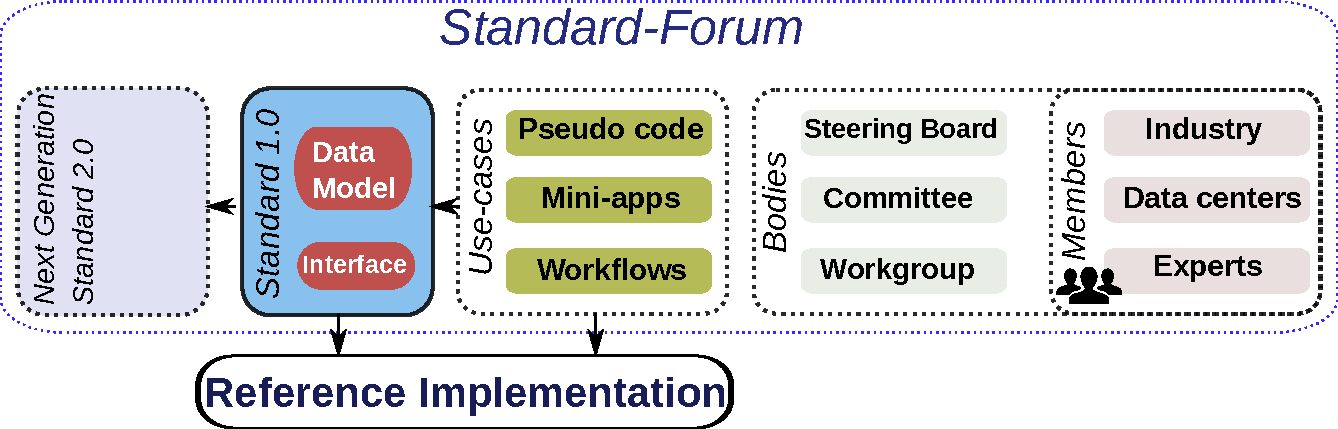
\includegraphics[width=\columnwidth]{standardization}
  \caption{Organization of the NGI Forum}
  \label{fig:standardization}
\end{figure}

\section{Conclusions}


\includegraphics[width=2cm]{ngi-logo}

\noindent\url{https://ngi.vi4io.org}


\end{document}
